\documentclass[a4paper, oneside]{article} 
\usepackage{tikz}
\usepackage{amsmath}
\usepackage{amsthm}
\usepackage{amssymb}
\usepackage{graphicx}
\usepackage[hidelinks]{hyperref}
\usepackage{enumitem}
\usepackage{nicefrac}
\usepackage{empheq}
\usepackage{xcolor}
\usepackage{array}
\usepackage{indentfirst}
\usepackage{enumitem}
\usepackage[fancysections, titlepage, pagenumber]{polytechnique}
\usepackage{float}

\theoremstyle{plain}
\newtheorem{theorem}{Theorem}
\setcounter{tocdepth}{2}

\newcommand{\castle}{C{\small.}A{\small.}S{\small.}T{\small.}L{\small.}E{\small.}}

\title[\castle{}]{Market Design Project: C.A.S.T.L.E.}
\subtitle{Capacity-Alligned Stable Teaching Location Engine\\
Tackling classroom allocation in Universities}
\author{Matthieu MINGUET}
\date{December 2024}

\begin{document}
\maketitle

\section{Executive Summary}
\pagebreak

\tableofcontents
\pagebreak

\section{Introduction}
The way the rooms are organized leads to inefficiencies, between professors who value and need different things. Some professors need to use boards to write specific, while others do not value such things. Moreover, the impact of the geographical positioning of the rooms relative to both the students and the teachers is something to take into consideration, or the proximity of the coffee machine, even the amount of stairs required to reach the room.
As such it is my belief that a new system designed around the principles of market design could lead to a more efficient allocation of the school’s resources, as well as collect valuable information term on term on what professors value and what type of classrooms they preconize.
\pagebreak

\section{Due Diligence}
\subsection{Current System at Ecole Polytechnique}
X currently operates a centralized room allocation system managed by the Registrar's office through a shared spreadsheet.
While the basic objective of assigning rooms to all classes is met, the system faces significant operational challenges.
The manual allocation process is time-consuming, requires frequent bargaining between departments, and often fails to meet teacher preferences and specific classroom needs.
Moreover, it does not provide a reporting of what the

The system's current stability relies heavily on the natural distribution of class sizes, particularly in the \textit{Cycle Ingénieur} program where enrollment decreases
from 550 students in first year to increasingly smaller specialized groups through second and third year. This pattern allows for predictable allocations, such as Poincare for large
lectures and smaller rooms for tutorials, especially when third-year students are off-campus. With the inversion of tutorials and lectures times based on the year, the system can support
the needs of the program.

However, mounting pressure from expanding masters and bachelor programs is straining this delicate balance. The competition for rooms,
especially between second and third-year needs, is intensifying. While the system functions now due to fortunate enrollment patterns,
it lacks the robustness to handle future growth and increasing complexity.

\subsubsection{Flaws in the current system}
In terms of market design, this system is a centralized dictatorship, as in a control economy where resources are allocated based on the sole criteria of class size. It's flaws which we will detail in the following table:\\

\begin{tabular}{|p{2.5cm}|p{10cm}|>{\centering\arraybackslash}p{2.5cm}|}
	\hline
	\textbf{Flaw}                                                                                 & \textbf{Description} & \textbf{Intensity} \\
	\hline
	Information Problem                                                                           &
	\begin{itemize}[leftmargin=*,nosep,topsep=0pt,partopsep=0pt,before=\vspace{-\baselineskip}]
		\item No preference elicitation
		\item Manual spreadsheet means no way to communicate preferences, constraints, or trade
	\end{itemize}     &
	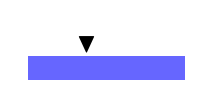
\begin{tikzpicture}
		\fill[blue!60] (0,0) rectangle (2,0.3);
		\node[anchor=center] at (0.75,0.45) {$\blacktriangledown$};
	\end{tikzpicture}                                                                                \\[2ex]
	\hline
	Matching Mechanism                                                                            &
	\begin{itemize}[leftmargin=*,nosep,topsep=0pt,partopsep=0pt,before=\vspace{-\baselineskip}]
		\item Single-Criterion Optimization: capacity matching
		\item Manual Coordination Cost: bargaining
		\item No formal Trading Mechanism: no beneficial trades
	\end{itemize}     &
	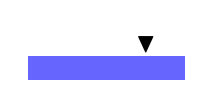
\begin{tikzpicture}
		\fill[blue!60] (0,0) rectangle (2,0.3);
		\node[anchor=center] at (1.5,0.45) {$\blacktriangledown$};
	\end{tikzpicture}                                                                                 \\[2ex]
	\hline
	Incentive Problems                                                                            &
	\begin{itemize}[leftmargin=*,nosep,topsep=0pt,partopsep=0pt,before=\vspace{-\baselineskip}]
		\item No strategic reporting: no formal way to express the preferences for rooms or features
		\item Lack of Price Mechanism: no way of quantifying preferences
	\end{itemize}  &
	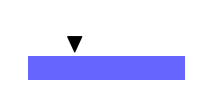
\begin{tikzpicture}
		\fill[blue!60] (0,0) rectangle (2,0.3);
		\node[anchor=center] at (0.6,0.45) {$\blacktriangledown$};
	\end{tikzpicture}                                                                                 \\[2ex]
	\hline
	Scalability                                                                                   &
	\begin{itemize}[leftmargin=*,nosep,topsep=0pt,partopsep=0pt,before=\vspace{-\baselineskip}]
		\item Brittle equilibrium: program change or growth could pose a threat to the current system
		\item Manual processing bottleneck
	\end{itemize} &
	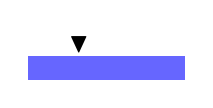
\begin{tikzpicture}
		\fill[blue!60] (0,0) rectangle (2,0.3);
		\node[anchor=center] at (0.65,0.45) {$\blacktriangledown$};
	\end{tikzpicture}                                                                                \\[2ex]
	\hline
	Efficiency problem                                                                            &
	\begin{itemize}[leftmargin=*,nosep,topsep=0pt,partopsep=0pt,before=\vspace{-\baselineskip}]
		\item No Optimization Algorithm
		\item Suboptimal Outcomes: room for Pareto improvements
		\item Resource Utilization: inefficient use of features and capabilities
	\end{itemize}    &
	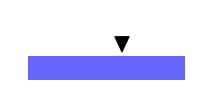
\begin{tikzpicture}
		\fill[blue!60] (0,0) rectangle (2,0.3);
		\node[anchor=center] at (1.2,0.45) {$\blacktriangledown$};
	\end{tikzpicture}                                                                                 \\[2ex]
	\hline
	Adaptation and flexibility                                                                    &
	\begin{itemize}[leftmargin=*,nosep,topsep=0pt,partopsep=0pt,before=\vspace{-\baselineskip}]
		\item Rigid system: changes mid-term can be difficult
		\item Limited feedback loop: for allocation and features
	\end{itemize}    &
	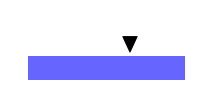
\begin{tikzpicture}
		\fill[blue!60] (0,0) rectangle (2,0.3);
		\node[anchor=center] at (1.3,0.45) {$\blacktriangledown$};
	\end{tikzpicture}                                                                                 \\[2ex]
	\hline
\end{tabular}
\linebreak

\vspace{0.05cm}

As we can see, while the current system has major flaws like the lack of a matching mechanism,
it still ensures all teachers have a room, and the school has functioned with this system for the past few years without any issues,
especially when the \textit{Cycle Ingénieur} program was the only program at the school.

\subsection{Current system at Clermont School of Business (Clermont SB)}
The Clermont SB has a similar system to Ecole Polytechnique, with a centralized room allocation and planning system. A dedicated member of staff is responsible
for managing the system in place: Program Directors submit room requirement and planning forms to the Planning Office, which then manually attributes the rooms based on the information provided,
and the availabilities of the rooms. These types of requirements include the number of rooms, the equipment, expected cohort size, and if the rooms need to be close to each other or not (for example for group work).
The number of variables makes it very difficult to find a solution satisfying all requirements of all courses.
While the system allows for inputs from the faculty, the major issue si that the large number of programs and the increasing number of students in each program
is making the system increasingly complex to manage by hand and is leading to inefficiencies and tensions in the allocation. Moreover, this system is quite slow and requires
a large amount of time to manage, which could be streamlined and better used elsewhere. Finally, the system is not transparent,
and the faculty does not have a clear understanding of how the rooms are allocated, while it also doesn't encourage truthful reporting of preferences.

\subsubsection{Flaws in the current system}
Similarly as what we did for Ecole Polytechnique, we have identified the following flaws in the current system at Clermont SB:\\

\begin{tabular}{|p{2.5cm}|p{10cm}|>{\centering\arraybackslash}p{2.5cm}|}
	\hline
	\textbf{Flaw}                                                                              & \textbf{Description} & \textbf{Intensity} \\
	\hline
	Information Problem                                                                        &
	\begin{itemize}[leftmargin=*,nosep,topsep=0pt,partopsep=0pt,before=\vspace{-\baselineskip}]
		\item Preference reporting through requirement forms
		\item Lack of transparency in allocation process
	\end{itemize} &
	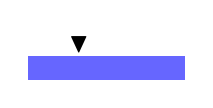
\begin{tikzpicture}
		\fill[blue!60] (0,0) rectangle (2,0.3);
		\node[anchor=center] at (0.65,0.45) {$\blacktriangledown$};
	\end{tikzpicture}                                                                             \\[2ex]
	\hline
	Matching Mechanism                                                                         &
	\begin{itemize}[leftmargin=*,nosep,topsep=0pt,partopsep=0pt,before=\vspace{-\baselineskip}]
		\item Manual attribution based on submitted forms
		\item Single-person decision making process
		\item No formal mechanism for resolving conflicts
	\end{itemize} &
	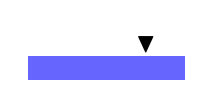
\begin{tikzpicture}
		\fill[blue!60] (0,0) rectangle (2,0.3);
		\node[anchor=center] at (1.5,0.45) {$\blacktriangledown$};
	\end{tikzpicture}                                                                              \\[2ex]
	\hline
	Incentive Problems                                                                         &
	\begin{itemize}[leftmargin=*,nosep,topsep=0pt,partopsep=0pt,before=\vspace{-\baselineskip}]
		\item No incentive for truthful preference reporting
		\item Lack of feedback mechanism
	\end{itemize} &
	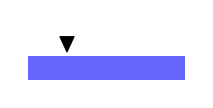
\begin{tikzpicture}
		\fill[blue!60] (0,0) rectangle (2,0.3);
		\node[anchor=center] at (0.5,0.45) {$\blacktriangledown$};
	\end{tikzpicture}                                                                              \\[2ex]
	\hline
	Scalability                                                                                &
	\begin{itemize}[leftmargin=*,nosep,topsep=0pt,partopsep=0pt,before=\vspace{-\baselineskip}]
		\item Growing complexity with increasing programs
		\item Rising student numbers strain current system
		\item Single point of failure (dedicated staff member)
	\end{itemize} &
	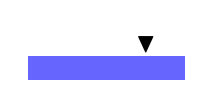
\begin{tikzpicture}
		\fill[blue!60] (0,0) rectangle (2,0.3);
		\node[anchor=center] at (1.5,0.45) {$\blacktriangledown$};
	\end{tikzpicture}                                                                              \\[2ex]
	\hline
	Efficiency problem                                                                         &
	\begin{itemize}[leftmargin=*,nosep,topsep=0pt,partopsep=0pt,before=\vspace{-\baselineskip}]
		\item Time-intensive manual process
		\item Inefficiencies in allocation
		\item Resource under-utilization due to information gaps
	\end{itemize} &
	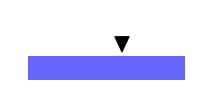
\begin{tikzpicture}
		\fill[blue!60] (0,0) rectangle (2,0.3);
		\node[anchor=center] at (1.2,0.45) {$\blacktriangledown$};
	\end{tikzpicture}                                                                              \\[2ex]
	\hline
	Adaptation and flexibility                                                                 &
	\begin{itemize}[leftmargin=*,nosep,topsep=0pt,partopsep=0pt,before=\vspace{-\baselineskip}]
		\item System struggles with program diversity
		\item Difficult to make mid-term adjustments
		\item Slow response to changing needs
	\end{itemize} &
	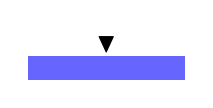
\begin{tikzpicture}
		\fill[blue!60] (0,0) rectangle (2,0.3);
		\node[anchor=center] at (1,0.45) {$\blacktriangledown$};
	\end{tikzpicture}                                                                                \\[2ex]
	\hline
\end{tabular}
\linebreak

As we can see, while this system offers more inputs from the different stakeholders, it is limited by the fact that it has to be
manually run, and an increasing number of programs and students compared to the number of rooms, or even more rooms could cause issues
regarding the length of the process and the fairness of the allocation.

\subsection{Market Sizing and existing solutions}
\subsubsection{Market Sizing}
Their are around $18500$ universities worldwide, representing around $250$m students. However, a new system such as \castle{} would be more suited to larger universities, especially in developed countries, where the number of students is higher, and the number of programs is more diverse.
As such, we estimate a theoretical market size of $5000$ universities, mainly in Europe and North America.
At first, this system would target around 80 universities in these markets, which considering their size could already impact upwards of $200000$ students.
Thus, \castle{} could bring an improvement over the current systems in place in these universities, and potentially be a game-changer in the way universities allocate their resources.

\subsubsection{Existing Papers}
Classroom allocation or time-tabling is a well-studied problem in the literature, with many papers proposing different solutions to the problem.
For example, Rivero, Escárcega, and Velasco (2021) proposed an Integer Linear Programming model for classroom assignment to tackle this issue, while other solutions
focus on graph coloring algorithms or genetic algorithms to allocate classrooms and timetables. In almost all cases, the solution to solve both
timetabling and classroom allocation is to decouple the two problems and solve them sequentially, as the classroom allocation algorithm generally output near 100\% utilization of the rooms,
which we will see is also the case for \castle{}.
The basic formulation of the problem for classroom allocation is as follows:
\begin{itemize}
	\item Let $x_{ij}$ be a binary variable where $i$ the classroom, $j$ the course and : $x_{ij} = 1$ if course $j$ is assigned to classroom $i$, $0$ otherwise.
	\item The objective function is : $\min \sum_{i,j} c_{ij}x_{ij}$ where $c_{ij}$ is the cost of assigning course $j$ to classroom $i$.
	\item $c_{ij}$ represents the cost of assigning class $j$ to classroom $i$, and can incorporate functions like room size mismatch, distance from the professor's department, equipment mismatch, etc.
\end{itemize}
The constraints are generally the following:
\begin{itemize}
	\item Single assignment constraint: $\sum_{i} x_{ij} = 1$ for all $j$
	\item Room capacity constraint: $\text{enrollment}_j \leq \text{capacity}_i \forall x_{ij} = 1$
\end{itemize}
In cases where timetables are also considered, the time $t$ is added as a third dimension to the problem, and the constraints are modified to include the time dimension (professor, room and student availabilities)
This formulation guarantees an optimal solution (if solvable) and is able to balance different objectives by weighting the $c_{ij}$, while being very flexible in terms of constraints and objectives.\\

However it is an NP-hard problem to solve and the solution space grows exponentially with the number of rooms, classes (and time slots). As an example, the Ecole Polytechnique has 76 rooms, around 65 to 70 classes at one time, for a complexity of $76^{70} \approx 10^{140}$, which is infeasible to solve with a brute force algorithm,
and we have not even considered the time dimension. Moreover, the model is static and can't easily handle dynamic changes.

Work exists to improve upon this by for example relaxing the strict constraints and adding a violation penalty, doing pre-processing to reduce the search space, or using heuristics to find a good solution in a reasonable time.
Other systems such as graph coloring exist, but they are also NP-hard, like the Integer Linear Programming model, and are generally less flexible as they have difficulty incorporating different objectives and soft constraints.\\

In conclusion, while significant academic work has been done on the subject of classroom allocation and timetabling, the problem remains complex and difficult to solve, especially in a dynamic environment like a university. Findings
from these papers are useful to understand the problem and the constraints, but a new approach is needed to tackle the problem in a more efficient way. We do keep in mind the idea of decoupling the
timetabling from the allocation, as \castle{} only focuses on the allocation part of the problem.

\section{Proposed Solution : \castle{}'s core principles}

The key objectives of \castle{} in light of the current systems and the existing literature are the following:
\begin{itemize}
	\item \textbf{Efficiency}: Maximizes room utilization and stakeholder satisfaction through optimal allocation of classrooms to courses.
	\item \textbf{Computability}: Delivers solutions within reasonable time frames on standard hardware, even at university scale.
	\item \textbf{Flexibility}: Adapts to diverse objectives and constraints while accommodating institution-specific requirements.
	\item \textbf{Transparency}: Ensures allocation decisions are understandable and promotes honest preference reporting.
	\item \textbf{Reliability}: Minimizes manual interventions by consistently producing near-complete room assignments across complex scenarios.
\end{itemize}

Moreover, we should also try to limit the time spent by faculty on this process, as it takes away from their time. \castle{} should also
not be based on any currency as this could cause problems with faculty and require more thought and time to use the system.
Based on the objectives of fitting the cohorts in the rooms and allowing the maximum amount of stakeholders such as faculty, students, and outside speakers
to benefit from the best and most sought after rooms, a cardinal parameter is to consider the "fill amount" of the rooms, or in other terms, to minimize
$\text{room}_{capacity} - \text{course}_{cohort size}$.

To achieve these objectives, two main algorithms were initially thought of:

\subsection*{You request my room, take it if you're bigger (YRMRTIYB)}
This is based on a similar idea as \textit{You request my house I get your turn} which is already based on the Top Trading Cycles (TTC) algorithm.
Each course would point towards the room they want, and the rooms towards their top choice of course. Then, the algorithm would find cycles of courses and rooms, and allocate the rooms to the courses in the cycle.
courses then point towards their next choices, and the algorithm continues until someone requests a room that is already taken, at which point if their cohort size is bigger, they get the turn of the first course.
Then the algorithm runs once more, and the cycle continues until all rooms are allocated.\\

The main problem of this algorithm is that stability is not guaranteed, which is a prerequisite for a long term allocation process. It does however bring strategy-proofness which is desirable to
avoid strategic reporting.

\subsection*{Deferred Acceptance Algorithm (DA)}
In this case, faculty members (or inversely rooms) would propose to a room (or inversely a faculty member) based on their preferences following the classic deferred acceptance algorithm.
This approach would guarantee stability, albeit without being inherently strategy-proof. Additionally, it is a well-know algorithm that has been implemented in many different contexts.
The final version of \castle{}'s algorithm is similar to that of "the Match" for medical students as it is a one-to-many matching.

\subsection{Matching algorithm implemented}
Room of identical types, such as rooms in the same corridors having the same equipment are grouped into a single type that represents them, order to  minimize the number of choices having
to be made by faculty members. As such their \textbf{preferences are for room types}. For the core algorithm we consider the fit function $f$. Finally, before running the algorithm, we consider the four following parameters
known: $\text{room}_{type}$, $\text{room}_{capacity}$, $\text{course}_{cohort size}$, and $\text{course}_{preferences}$.
\begin{enumerate}
	\item Courses propose to their top choice of room type based on their preferences. We then run the steps 2 to 4 for each room type separately.
	\item All proposals to a type are grouped, including any courses already tentatively allocated in the rooms.
	\item In order of increasing capacity, rooms tentatively choose the course corresponding to $\underset{course}{\min} f(course, room)$,
	      and it is removed from the list of proposals.
	\item Once all rooms in the type have chosen the remaining courses are sent back to the global proposal pool, or their are no remaining proposals in this type.
	\item The remaining courses change their current choice of room type to the next one and go back to step 1.
	\item The algorithm stops when all courses have been allocated a room, or the remaining courses have tried all their choices.
\end{enumerate}

\subsection{Properties of the algorithm}
The proposed algorithm has multiple desirable properties for our market design problem.
\subsubsection{Definitions and Notation}
Let us define:
\begin{itemize}
    \item $C = \{c_1, ..., c_n\}$: Set of courses
    \item $R = \{r_1, ..., r_m\}$: Set of rooms
    \item $T = \{t_1, ..., t_k\}$: Set of room types
    \item $P$: the maximum number of preferences per course ($P \leq T$)
    \item $\succ_c$: Preference relation for course $c$ over room types
    \item $\mu$: A matching function $C \rightarrow R \cup \{\emptyset\}$
    \item $s(c)$: Size of course $c$
    \item $cap(r)$: Capacity of room $r$
    \item $type(r)$: Type of room $r$
\end{itemize}
\subsubsection{Computability}
Let us define the following variables:, $C$ the number of courses to be allocated, $R$ the number of rooms, $T$: the room types,
$P$ the maximum number of preferences per course ($P \leq T$)

The allocation process can be visualized as the following flowchart:
\begin{enumerate}
	\item For each unmatched course ($O(C)$):
	      \begin{itemize}
		      \item Group proposals by type: $O(C)$
		      \item For each room type ($O(T)$):
		            \begin{itemize}
			            \item Sort rooms by capacity: $O(R \log R)$
			            \item For each room, evaluate all available courses: $O(R \cdot C)$
		            \end{itemize}
	      \end{itemize}
\end{enumerate}

The algorithm has a $\boxed{\text{worst-case time complexity of: } O(C \cdot T \cdot (R \log R + R \cdot C))}$ and a space complexity of $O(R + C)$.

However, in practical applications, several factors contribute to better average-case performance:
\begin{enumerate}
	\item Most courses are matched in early iterations, reducing the effective number of rounds from $O(C)$ to approximately $O(P)$
	\item Room types $T$ is a small constant (approximately 10 in our implementation), and $P \leq T$.
	\item With a relatively small number of rooms ($R < 1000$), the room sorting component becomes nearly linear: $O(R \log R) \approx O(R)$
\end{enumerate}

As such, the results are an $\boxed{\text{average-case time complexity of simply } O(C \cdot R)}$, and space complexity $O(R + C)$. This is a significant improvement and
enables the algorithm to run in a reasonable time frame on standard hardware, even at university scale. 
Empirical evidence from our implementation supports this analysis. With a typical scenario of 70 courses and 70 rooms and spread out preferences, the algorithm completes in 150-300 allocation steps,
with most courses being matched within their first three preferences.

\subsubsection{Stability Analysis}
\begin{theorem}[Stability]
\castle{} allocation mechanism produces a stable matching.
\end{theorem}

\begin{proof}
Suppose, for contradiction, that the matching $\mu$ is unstable. Then there exists a blocking pair $(c, r)$ where:
$c$ prefers $r$ to its current assignment $\mu(c)$ and $r$ prefers $c$ to its current occupant $\mu^{-1}(r)$.
However, by construction of the algorithm:
\begin{enumerate}
    \item If $type(r) \succ_c type(\mu(c))$, then $c$ would have proposed to rooms of type $type(r)$ before $type(\mu(c))$
    \item Within each type, rooms are assigned to best-fitting courses based on capacity utilization
    \item If $s(c) \leq cap(r)$ and $capafit(r,c) < capafit(r,\mu^{-1}(r))$, then $r$ would have been assigned to $c$ in the per-type processing phase
\end{enumerate}
Thus contradicting the existence of a blocking pair, proving stability.
\end{proof}

\subsubsection{Pareto Efficiency}
\begin{theorem}[Pareto Efficiency]
\castle{} allocation produces a Pareto efficient matching among stable matchings within each type.
\end{theorem}

\begin{proof}
Consider a matching $\mu$ produced by the algorithm. Suppose, for contradiction, that there exists another stable matching $\mu'$ that Pareto dominates $\mu$.
This means:
\begin{enumerate}
    \item $\forall c \in C$: $type(\mu'(c)) \succeq_c type(\mu(c))$
    \item $\exists c^* \in C$: $type(\mu'(c^*)) \succ_{c^*} type(\mu(c^*))$
\end{enumerate}
For types processed in round $k$, let $C_k$ be the set of courses assigned in that round. The algorithm maximizes:
$$\sum_{c \in C_k} capafit(c, \mu(c))$$
Therefore, any improvement for $c^*$ would necessarily worsen the fit for some other course in the same round, contradicting Pareto dominance.
\end{proof}

\subsubsection{Strategy-proofness Analysis}

While the classic deferred acceptance algorithm is not generally strategy-proof, \castle{}'s variant has interesting properties that make it difficult to manipulate.
\begin{theorem}[Limited Manipulability]
Capacity constraints, Multi-dimensional preferences, Information asymmetry limit manipulability of the mechanism.
\end{theorem}

\begin{proof}
Consider a course $c$ attempting to manipulate its preference list $\succ_c$. For successful manipulation:
\begin{enumerate}
    \item $c$ must know:
        \begin{itemize}
            \item Preferences of other courses: $\{\succ_{c'}\}_{c' \in C\setminus\{c\}}$
            \item Sizes of other courses: $\{s(c')\}_{c' \in C\setminus\{c\}}$
            \item Room capacities: $\{cap(r)\}_{r \in R}$ which he does know as it is public information
        \end{itemize}
    \item $c$ must find a preference list $\succ_c'$ such that:
        $$type(\mu'(c)) \succ_c type(\mu(c))$$
        where $\mu'$ is the matching under manipulated preferences
\end{enumerate}
\end{proof}

\paragraph{Practical Implications}

In conclusion, theoretical properties have important practical implications:

\begin{enumerate}
    \item Stability ensures no course-room pair has incentive to deviate and should allow for a long-term deployment
    \item Pareto efficiency guarantees no wasteful assignments within types, maximizing room utilization and stakeholder satisfaction
    \item Limited manipulability reduces gaming concerns in practical deployments, promoting honest preference reporting and makes it easier to understand the preferences of the faculty
    \item Thus, the mechanism balances competing objectives:
        \begin{itemize}
            \item Course preferences over room types
            \item Efficient room capacity utilization
            \item Fair allocation among courses
        \end{itemize}
\end{enumerate}

Hence, the proposed mechanism is well-suited to the challenges posed by university classroom allocation, offering a robust, efficient, easy to use solution, 
that offers good properties for the stakeholders. It manages to achieve computability by restricting the tested combinations to those asked by the faculty
in the Gale-Shapley algorithm, which also guarantees stability and Pareto efficiency. Finally, it is not strategy-proof, but the limited manipulability 
encourages honest reporting of preferences and reduces the risk of gaming the system.

\section{Implementation and Testing}
\subsection{Implementation}

The algorithm was implemented in Java, leveraging object-oriented programming principles to model the problem and solution effectively.
Moreover, it allows for clear organization of the code and easy extension and modification of the algorithm with different parameters, fit functions,
rooms or constraints through the use of abstract classes and interfaces. This creates a modular and flexible environment for coding and testing the algorithm.
Most importantly, the execution speed of java versus python is nearly 100 times faster, which eases the use of the algorithm on a large scale and quick changes.
This is achieved without the need for complex parallelization or optimization, as the algorithm is already efficient enough to run on a standard laptop.
On a scenario of the size of Ecole Polytechnique, the algorithm runs in around 10 milliseconds, which is more than acceptable for a near real-time allocation process.
The code structure and key elements are detailed in the annex. The main classes are the allocation algorithm, all the objects representing the courses, rooms,
and room types, and the fit function.


\end{document}